\section{friendship}

\subsection{access modifiers}

\begin{frame}[fragile]{access modifiers}
	Wir kennen bereits für die member von Klassen (\verb|class|, \verb|struct|, \verb|union|).
	Wenn man sagt, eine Klasse habe Zugriff auf einen member, so bedeutet dies, dass die member dieser Klasse diesen Zugriff besitzten (z.B. member functions).
	
	\pause
	
	\begin{block}{Zugriffskontrolle für member}
		Zugriff für member in einer Klasse A für:
		\begin{itemize}[<+->]
			\item \verb|public| -- jeden
			\item \verb|protected| -- nur die Klasse A selbst und deren Kindklassen
			\item \verb|private| -- nur die Klasse A selbst
		\end{itemize}
	\end{block}
\end{frame}

\begin{frame}{encapsulation \& information hiding}
	\begin{itemize}[<+->]
		\item Faustregel: Alles so weit wie möglich schützen!
		\item data member i.d.R. private
		\item nur sichere, in sich geschlossene Funktionen public
	\end{itemize}
\end{frame}

\begin{frame}{friendship}
	Friendship erlaubt eine feinere Kontrolle über member access:
	
	\alt<2->
	{% on slide 2
		image: friendship
		%\includegraphics[\textwidth]{images/friendship}
	}{% on slide 1
		image: non-friendship
		%\includegraphics[\textwidth]{images/non-friendship}
	}
\end{frame}


\subsection{forward declarations}

\begin{frame}[fragile]{Deklaration und Definition}
	\begin{block}{Standard, 3.1}
		Eine Deklaration führt einen Namen ein (in eine translation unit).
		Eine Deklaration ist zugleich eine Definition, außer:
		\begin{itemize}[<+->]
			\item es ist der Name einer Funktion oder Klasse und es fehlt der Körper {\tiny (das zwischen den geschweiften Klammern) }
			\item die Deklaration enthält einen linkage-specifier (\verb|static|, \verb|extern|) aber weder einen Körper noch eine Initialisierung
			\item es ist die Deklaration einer Klassenvariablen
		\end{itemize}
	\end{block}
	
	\vspace{1em}
	
	\uncover<+->
	{
		Eine Deklaration sagt: es gibt einen Namen
		Eine Definition beschreibt, was genau mit dem Namen bezeichnet wird.
	}
\end{frame}

\begin{frame}[fragile]{Deklaration und Definition: Beispiele}
	\footnotesize
	\begin{lstlisting}[language=C++, basicstyle=\footnotesize, numbers=left, numberstyle=\tiny\color{gray}, tabsize=6, xleftmargin=2em]
int a; // defines a
extern const int c = 1; // defines c
int f(int x) { return x+a; } // defines f and defines x
struct S { int a; int b; }; // defines S, S::a, and S::b
struct X { // defines X
int x; // defines nonstatic data member x
static int y; // declares static data member y
X(): x(0) { } // defines a constructor of X
};
int X::y = 1; // defines X::y
enum { up, down }; // defines up and down
namespace N { int d; } // defines N and N::d
namespace N1 = N; // defines N1
X anX; // defines anX

extern int a; // declares a
extern const int c; // declares c
int f(int); // declares f
struct S; // declares S
typedef int Int; // declares Int
extern X anotherX; // declares anotherX
using N::d; // declares N::d
	\end{lstlisting}
\end{frame}

\begin{frame}[fragile]{Wozu?}
	unqualified name lookup (Standard, 3.4.1:4-8)
	
	Ein Name benutzt direkt in einem namespace muss zuvor deklariert sein.
	\begin{lstlisting}[language=C++, basicstyle=\footnotesize, numbers=left, numberstyle=\tiny\color{gray}, tabsize=6, xleftmargin=2em]
class X { };
namespace nsp {
	class Y { };
	void bar(X x);
	void bar(Y y);
}
	\end{lstlisting}
\end{frame}

\begin{frame}[fragile]{functions}
	\begin{block}{Voraussetzungen an Funktionen beim Aufruf (Standard, 3.2:3, 3.5:2)}
		\begin{itemize}
			\item Der Name muss zuvor deklariert sein.
			\item Es muss (irgendwo) eine entsprechende Definition geben.
		\end{itemize}
	\end{block}
	
	\begin{block}{Syntax}
		\begin{columns}[t]
			\column{0.4\textwidth}
			\emph{translation unit 1}
			\vspace{0.5em}
			\begin{lstlisting}[language=C++, basicstyle=\footnotesize, numbers=left, numberstyle=\tiny\color{gray}, tabsize=6, xleftmargin=2em]
void foo(int i);
void bar() { foo(42); }
			\end{lstlisting}
			
			\column{0.4\textwidth}
			\emph{beliebige translation unit}
			\vspace{0.5em}
			\begin{lstlisting}[language=C++, basicstyle=\footnotesize, numbers=left, numberstyle=\tiny\color{gray}, tabsize=6, xleftmargin=2em]
#include <iostream>
void foo(int i) { std::cout << i; }
			\end{lstlisting}
		\end{columns}
	\end{block}
\end{frame}

\begin{frame}[fragile]{Incomplete Types}
	Eine Klasse, die nur deklariert aber nicht definiert wurde, ist ein \emph{incomplete type}.
	Es dürfen keine »Dinge« mit incomplete type angelegt werden.
	Es dürfen sehr wohl Referenzen und Pointer auf incomplete types angelegt werden.
	
	Ein Pointer auf einen incomplete type ist modifizierbar, aber nicht dereferenzierbar.
	
	Bevor man einen Pointer/Referenz nutzt, sollte der type completed sein (definiert). Sonst darf man quasi nichts mit dem Pointer/Referenz tun. Siehe Standard, 3.2:4, 5.2.2:4, 5.3.1:4, 5.7:1, 8.3.5:6
	
	\begin{lstlisting}[language=C++, basicstyle=\footnotesize, numbers=left, numberstyle=\tiny\color{gray}, tabsize=6, xleftmargin=2em]
		struct X;
		void foo(X); // alt: void foo(X x);
		
		struct X { int m; };
		void foo(X x)
		{
			x.m = 42;
		}
	\end{lstlisting}
\end{frame}

\begin{frame}[fragile]{classes, types}
	\begin{block}{Syntax}
		\begin{columns}[t]
			\column{0.4\textwidth}
			\begin{lstlisting}[language=C++, basicstyle=\footnotesize, numbers=left, numberstyle=\tiny\color{gray}, tabsize=6, xleftmargin=2em]
 class A;
struct B;
 union C;
  enum D;
			\end{lstlisting}
			
			\column{0.4\textwidth}
			\begin{lstlisting}[language=C++, basicstyle=\footnotesize, numbers=left, numberstyle=\tiny\color{gray}, tabsize=6, xleftmargin=2em]
 class A { int m; };
struct B { void doit(); };
 union C { int m; char c; };
  enum D { X, Y, Z };
			\end{lstlisting}
		\end{columns}
	\end{block}
	
	\pause
	
	Wozu verwenden?
	\pause
	Für gegenseitige Abhängigkeiten oder auch information hiding!
	\begin{lstlisting}[language=C++, basicstyle=\footnotesize, numbers=left, numberstyle=\tiny\color{gray}, tabsize=6, xleftmargin=2em]
class A;
class B;
class B { A* getA(); };
class A { void doB(B*); };
	\end{lstlisting}
\end{frame}


\subsection{friend}

\begin{frame}[fragile]{Syntax}
	\begin{lstlisting}[language=C++, basicstyle=\footnotesize, numbers=left, numberstyle=\tiny\color{gray}, tabsize=6, xleftmargin=2em]
struct B;
void globalFunc(B b);
struct A { void foo(B b); };

struct B {
	// public, private, protected or nothing at all
	friend class A;
	friend void globalFunc();
private:
	int m;
	void doInternal();
};
	\end{lstlisting}
	
	\pause
	
	\begin{block}{Syntax (Standard, 11.4)}
		Friendship gewährt man durch eine Deklaration in der Klassen-\emph{member-specification} mit \emph{friend-specifier} und für einen Typen mit \emph{elaborated-type-specifier} (7.1.5.3).
	\end{block}
\end{frame}

\begin{frame}[fragile]{Wirkung}
	Siehe Standard, 11.4.
	Hauptsächlich: man darf in member functions der befreundeten Klasse auf private member der Freundschaft-gewährenden Klasse zugreifen.
	
	\begin{block}{Beispiel}
		\begin{columns}[t]
			\column{0.4\textwidth}
			\begin{lstlisting}[language=C++, basicstyle=\footnotesize, numbers=left, numberstyle=\tiny\color{gray}, tabsize=6, xleftmargin=2em]
struct B {
	// public, private, protected or nothing at all
	friend class A;
	friend void globalFunc();
private:
	int m;
	void doInternal();
};
			\end{lstlisting}
			
			\column{0.4\textwidth}
			\begin{lstlisting}[language=C++, basicstyle=\footnotesize, numbers=left, numberstyle=\tiny\color{gray}, tabsize=6, xleftmargin=2em]
void globalFunc(B b)
{
	b.doInternal();
}
void A::foo(B b)
{
	b.m = 42;
	b.doInternal();
}
			\end{lstlisting}
		\end{columns}
	\end{block}
\end{frame}

\begin{frame}{Hinweise}
	\begin{itemize}[<+->]
		\item Friendship wird nicht vererbt!
		\item Friendship ist nicht transitiv!
	\end{itemize}
\end{frame}
